\documentclass{article}
% Change "article" to "report" to get rid of page number on title page
\usepackage{amsmath,amsfonts,amsthm,amssymb}
\usepackage{setspace}
\usepackage{fancyhdr}
\usepackage{lastpage}
\usepackage{extramarks}
\usepackage{chngpage}
\usepackage{soul}
\usepackage[usenames,dvipsnames]{color}
\usepackage{graphicx,float,wrapfig}
\usepackage{ifthen}
\usepackage{listings}
\usepackage{courier}
\usepackage{upquote}

\definecolor{MyDarkGreen}{rgb}{0.0,0.4,0.0}
\newcommand{\ComplexUnit}{\ensuremath{\mathrm{i}}}

% For faster processing, load Matlab syntax for listings
\lstloadlanguages{Python}%
\lstset{language=Python,
        frame=single,
        basicstyle=\small\ttfamily,
        keywordstyle=[1]\color{Blue}\bf,
        keywordstyle=[2]\color{Purple},
        keywordstyle=[3]\color{Blue}\underbar,
        identifierstyle=,
        commentstyle=\usefont{T1}{pcr}{m}{sl}\color{MyDarkGreen}\small,
        stringstyle=\color{Purple},
        showstringspaces=false,
        tabsize=5,
        % Put standard Python functions not included in the default
        % language here
        morekeywords={},
        % Put Python function parameters here
        morekeywords=[2]{},
        % Put user defined functions here
        morekeywords=[3]{},
        morecomment=[l][\color{Blue}]{...},
        numbers=left,
        firstnumber=1,
        numberstyle=\tiny\color{Blue},
        stepnumber=5
        }

% In case you need to adjust margins:
\topmargin=-0.45in      %
\evensidemargin=0in     %
\oddsidemargin=0in      %
\textwidth=6.5in        %
\textheight=9.0in       %
\headsep=0.25in         %

%% % Homework Specific Information
%% \newcommand{\hmwkTitle}{One}
%% \newcommand{\hmwkSubTitle}{Two}
%% \newcommand{\hmwkDueDate}{Three}
%% \newcommand{\hmwkClass}{Four}
%% \newcommand{\hmwkClassTime}{Five}
%% \newcommand{\hmwkClassInstructor}{Six}
%% \newcommand{\hmwkAuthorName}{Seven}

%% % Setup the header and footer
\pagestyle{fancy}                                                       %
%% \lhead{\hmwkAuthorName}                                                 %
%% \chead{\hmwkClass\ (\hmwkClassInstructor\ \hmwkClassTime): \hmwkTitle}  %
%% \rhead{\firstxmark}                                                     %
\lfoot{\lastxmark}                                                      %
\cfoot{}                                                                %
\rfoot{Page\ \thepage\ of\ \protect\pageref{LastPage}}                  %
\renewcommand\headrulewidth{0.4pt}                                      %
\renewcommand\footrulewidth{0.4pt}                                      %

\title{Coherent population trapping with pulsed laser,\\the notes}
\author{Greg}
\date{version 0.1, \today}

\begin{document}
\begin{spacing}{1.1}
\maketitle
% Uncomment the \tableofcontents and \newpage lines to get a Contents page
% Uncomment the \setcounter line as well if you do NOT want subsections
%       listed in Contents
%% \setcounter{tocdepth}{1}
\tableofcontents
\newpage


\section{Introduction}
This note supposed to summarize the current status of the Bloch-equation calculation towards explaining the frequency-comb Coherent Population Trapping (CPT) experiment. It starts in the very beginning, because there is a lot to learn. For most of the calculations I adopt notation that is convenient for me. If I have to convert from the notation of e.g. a paper, I give the method of conversion too. 

A single element of the a density matrix is a complex number. For many calculations it is more convenient to use only real numbers, thus we separate the real an imaginary component.
\begin{equation}
\rho_{kl} = x_{kl} + \ComplexUnit y_{kl}
\end{equation}
The diagonal elements of the density matrix are called populations, while the off-diagonals are the coherences. Since the density matrix has is Hermitian, the populations are real numbers, while the coherences are generally complex.

The simplest Bloch equations are written in the following form, for the time derivative of the  populations, and the real / imaginary part of the coherences:
\begin{subequations}
\begin{align}
\dot x_{jj} &= \sum_{l=1}^N (2 M_{lj} y_{jl} + A_{jl} x_{ll}) - \gamma_j x_{jj} \\
\dot x_{jk} &= \sum_{l=1}^N (- M_{jl} y_{lk} + y_{jl} M_{lk}) - x_{jk} \left(\frac{\Gamma_j + \Gamma_k + \Gamma_{L,jk}}{2}\right) + y_{jk} \Delta_{jk} \\
\dot y_{jk} &= \sum_{l=1}^N (  M_{jl} x_{lk} - x_{jl} M_{lk}) - y_{jk} \left(\frac{\Gamma_j + \Gamma_k + \Gamma_{L,jk}}{2}\right) - x_{jk} \Delta_{jk}
\end{align}
\end{subequations}


\section{Repeating results from other papers}

\subsection{Basic three level system}
From my precious group, Matt McDonnel's thesis \cite{McDonnell2003}
Figures 4.3, 4.5, 4.6, 4.7. Correction, time is scaled as $1/\Gamma$, not as in the thesis claimed as $2\pi/\Gamma$.

\begin{figure}
\begin{center}
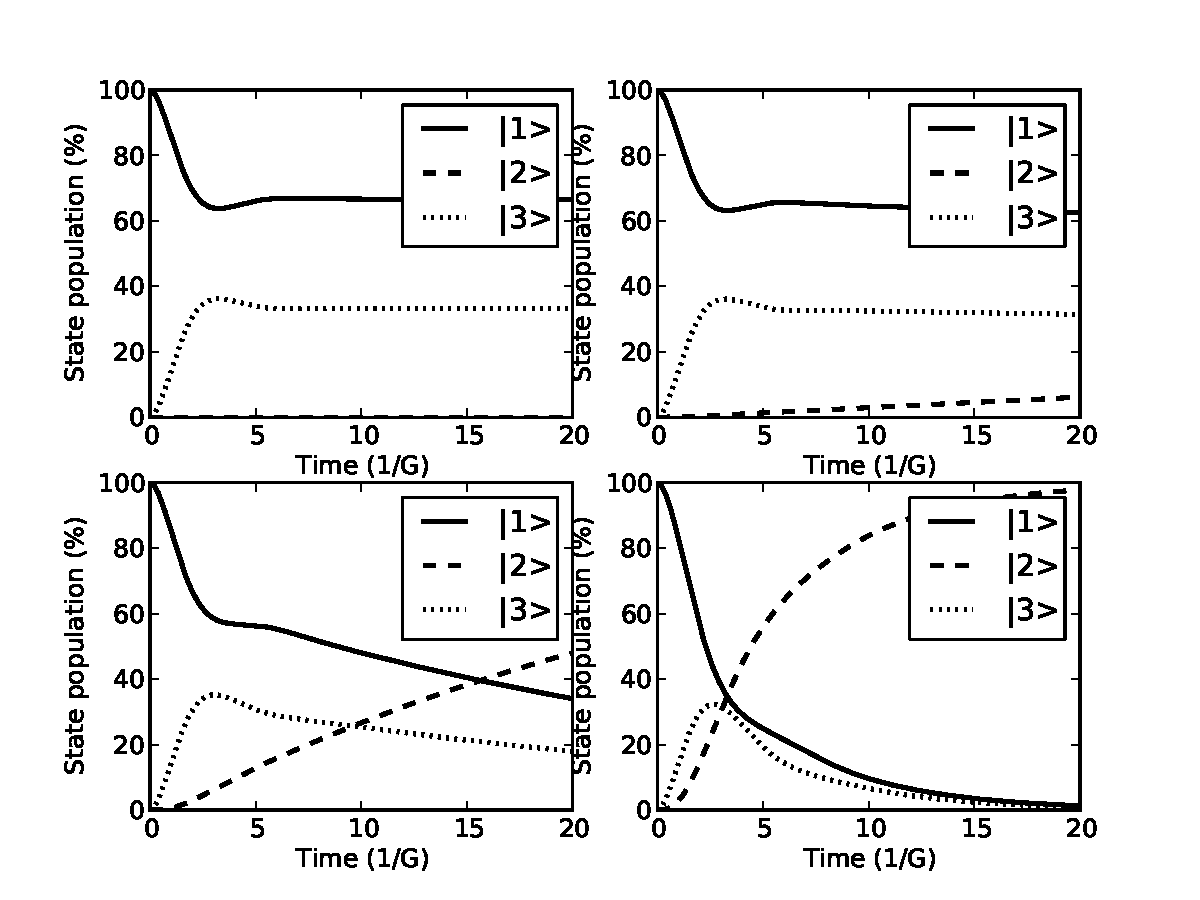
\includegraphics[width=0.65\textwidth]{figures/matt43.pdf}
\caption{Reproducing Figure 4.3 from \cite{McDonnell2003}}
\label{fig:matt43}
\end{center}
\end{figure}

\begin{figure}
\begin{center}
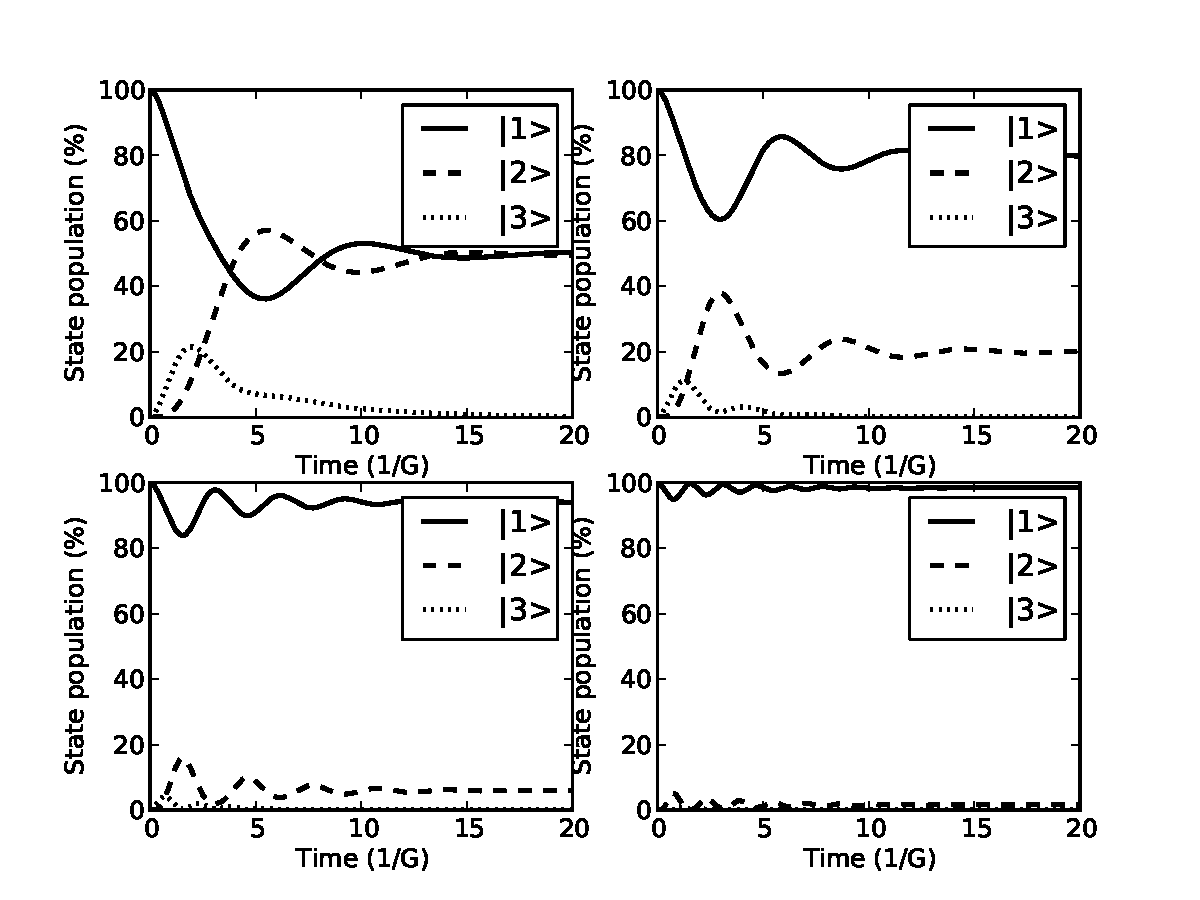
\includegraphics[width=0.65\textwidth]{figures/matt45.pdf}
\caption{Reproducing Figure 4.5 from \cite{McDonnell2003}}
\label{fig:matt43}
\end{center}
\end{figure}

\begin{figure}
\begin{center}
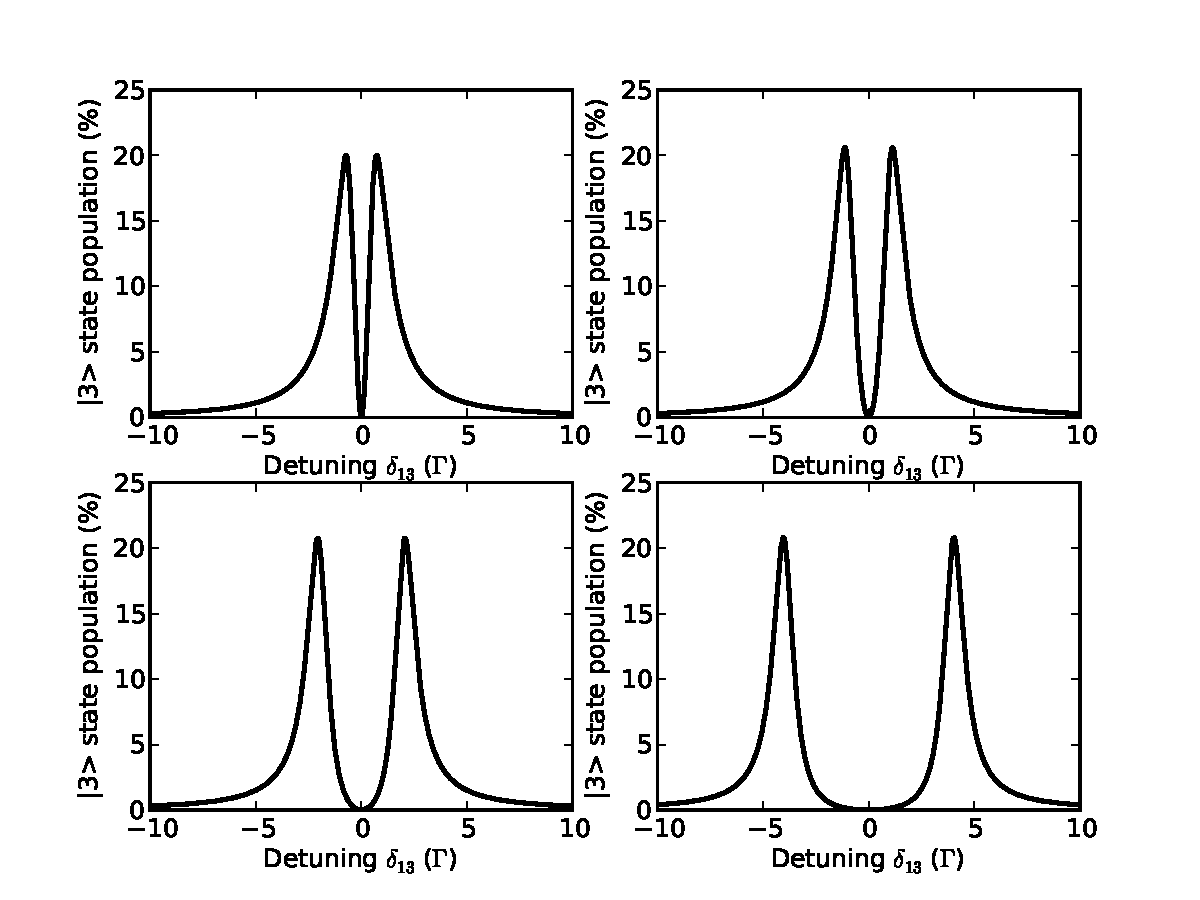
\includegraphics[width=0.65\textwidth]{figures/matt46.pdf}
\caption{Reproducing Figure 4.6 from \cite{McDonnell2003}}
\label{fig:matt43}
\end{center}
\end{figure}

\begin{figure}
\begin{center}
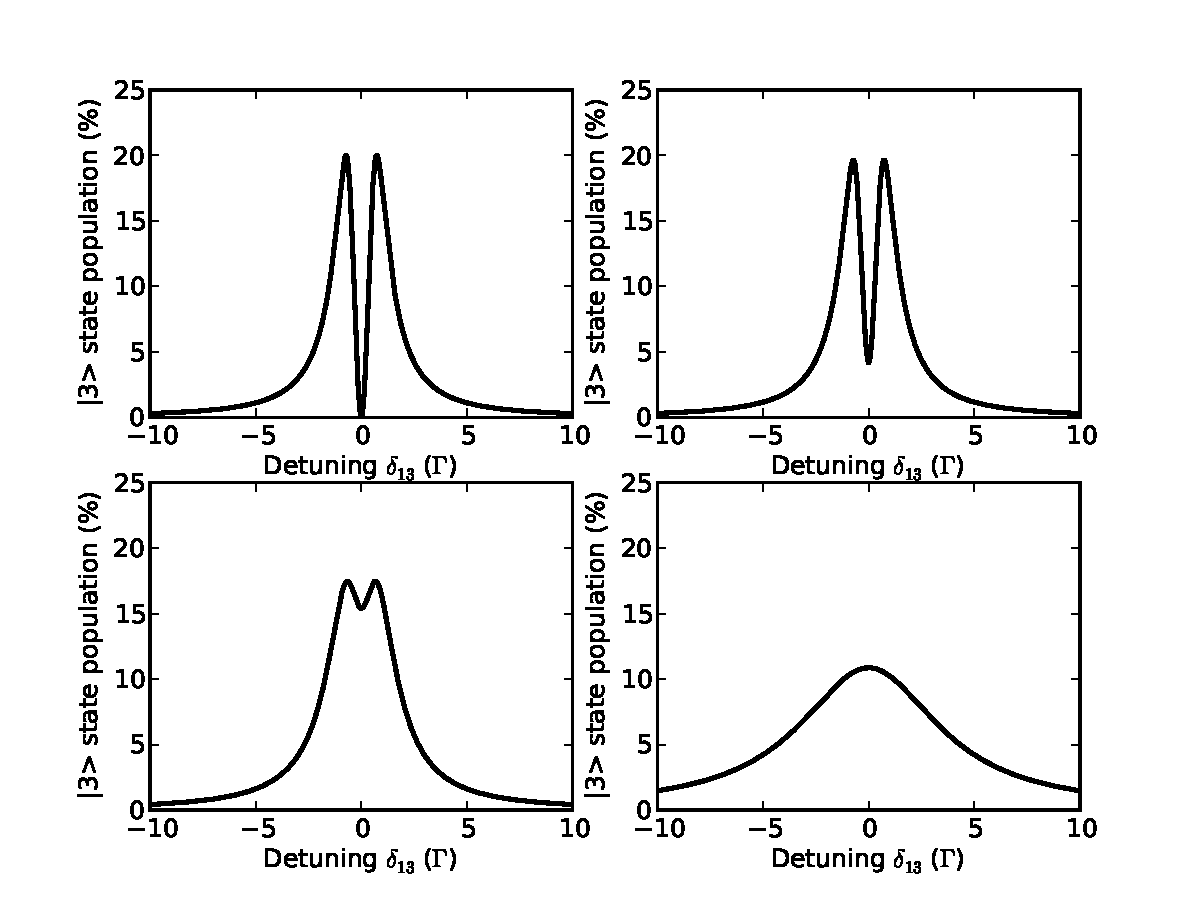
\includegraphics[width=0.65\textwidth]{figures/matt47.pdf}
\caption{Reproducing Figure 4.7 from \cite{McDonnell2003}}
\label{fig:matt43}
\end{center}
\end{figure}

\subsection{CW + pulsed system}
This is \cite{Soares2010}, describing mixed, CW + pulsed laser EIT case.

\subsection{Pulsed rubidium system}
This is \cite{Arissian2006}, describing a mode-locked $^{87}$Rb experiment.


\section{New calculations}
%% now... \cite{Berman1986}
%% \begin{lstlisting}[label=test,caption={[short] caption text }]
%% from numpy import *
%% import pylab as pl

%% data = loadtxt('filename.txt')
%% time = data[:, 0]
%% fluo = data[:, 1]
%% pl.plot(time, fluo, 'k-')
%% pl.xlabel('Time (s)')
%% pl.ylabel('Fluorescence (A.U.)')
%% pl.show()
%% \end{lstlisting}

\subsection{Things to check in the futre}
\begin{itemize}
\item Full cesium system
\item Magnetic field
\item Buffer gas effects, shift, broadening/narrowing
\item Higher energy levels for multi-photon processes
\end{itemize}

\newpage
\addcontentsline{toc}{section}{Bibliography}
\bibliographystyle{apalike}
\bibliography{physics_all}

\end{spacing}
\end{document}

%%%%%%%%%%%%%%%%%%%%%%%%%%%%%%%%%%%%%%%%%%%%%%%%%%%%%%%%%%%%%
